\section{Experimentation Setup}
In order to find the best method for learn the Kick Motion, we tested several techniques to compare them and find out that one which converges faster and results in the better and more robust kick. In the next subsections, we will describe each of the methods evaluated in this work.

\subsection{Hybrid Learning Model -- HLM}
In the Hybrid Learning Model (HLM), the training process occurs in two phases. The first one, a supervised learning phase, we learn the keyframe used by using a neural network, reproducing almost the same motion that we already had previously. The intuition behind this is if the agent starts from a good initial point in the optimization problem, it could be easier to get better results applying the gradient in the neighborhood of that point. The reward starts with a good value and the starting motion is well defined. Otherwise, if the optimization starts in a random point, it could be impossible to reach a good motion and probably the agent will get stuck in a local optima. This idea is shown in Figure \ref{optimization_intuition}.

\begin{figure}[!htbp]
	\centering
	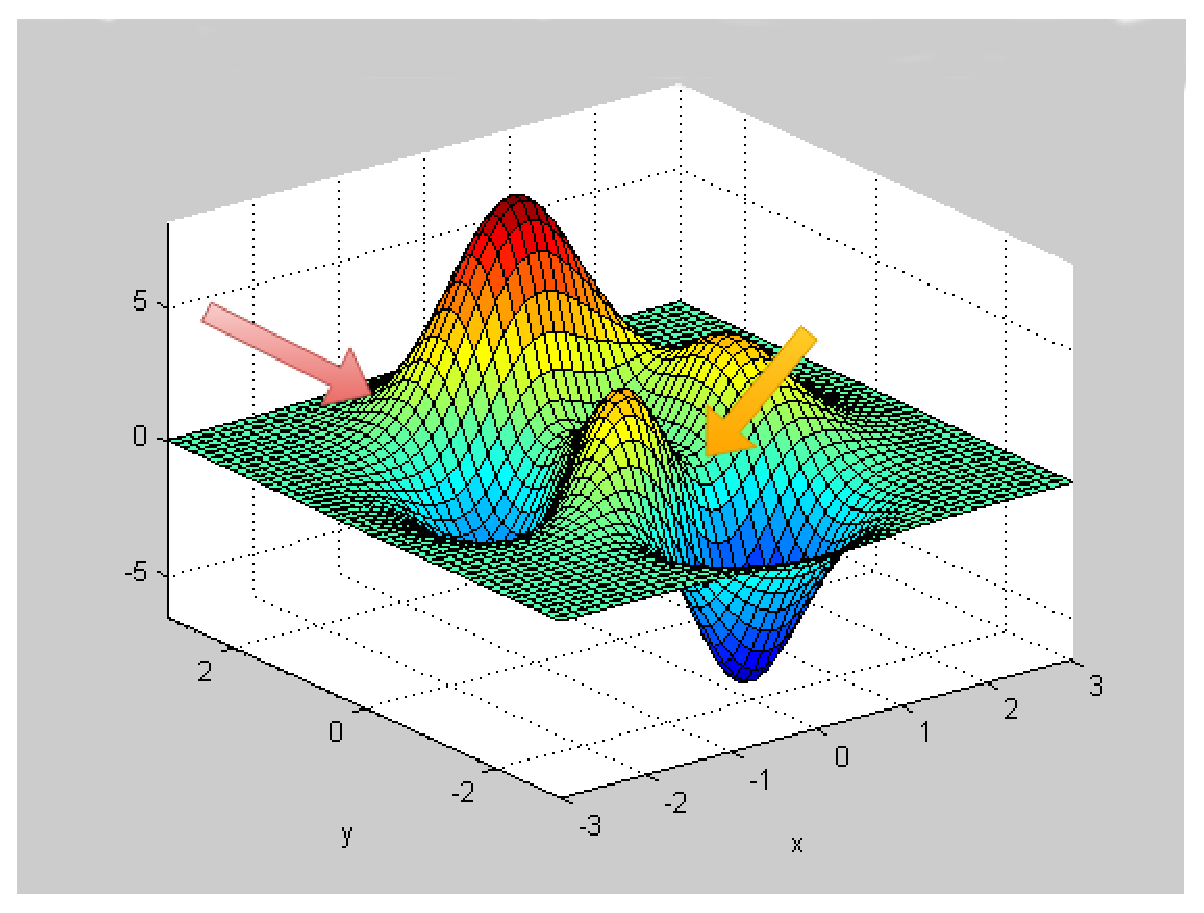
\includegraphics[width=0.5\textwidth]{Cap5/optimization_final.eps}
	\caption{In the hybrid model, we can ensure the starting point is near of the optimal solution (orange arrow); otherwise, the starting point can be bad and harder to optimize (red arrow).}
	\label{optimization_intuition}
\end{figure}

\subsection{Reinforcement with Naive Reward - RNR }
In this learning model, we just use reinforcement learning with a simple and directly reward. As our task is related to kick the ball, the "naive" reward is composed by its velocities after the kick motion, as shown in \ref{naive_reward}, where $s$, $v$ and $u$ are actual state, the vector of velocity and weight parameters, respectively. We call it naive because we don't pass to the learning model any idea of how the motion have to be performed - just what we expect to have as final objective. 

It is important to highlight that the techniques described could be used jointly as building blocks of a more labored model.

\begin{equation}
R(s) = u^{T}v
\label{naive_reward}
\end{equation}

\subsection{Reinforcement with Reference Reward - RRR }
In this learning model we add a term that compares the actual performance with a reference motion, as shown in \ref{complete_reward}:

\begin{equation}
R(s) = w_{ref}^{T}r
\label{complete_reward}
\end{equation}

In this equation, $w_{ref}$ are weight parameters for each joint and $r$ is the absolute value of the difference between joint values in that state and the reference (equation \ref{diffjoints}).

\begin{equation}
r(\theta, \theta_{0}) = \lVert\theta - \theta_{0}\rVert
\label{diffjoints}
\end{equation}

The intuition behind this weight parameters is because we have some joints more important than others. For example, some joints from the leg that kicks the ball themselves could collapse the whole motion if the error is high. On the other hand, joints from the neck are not so important to the kick. Therefore, it's natural to penalize differently in each case.

Lastly, the reference motion used was the keyframe kick previously mentioned and also used in HLM.


\subsection{Reinforcement with Initial State Distribution - RISD}

The Initial State Distribution is a technique related to where the episode starts to collect data to use in the learning. Without this technique, all episodes start in the beginning of the motion. However, the problem of this strategy is because the policy is forced to learn the motion in a sequential manner, first learning the early phases of the motion, and then incrementally progressing towards the later phases. This can be problematic for the kick motion. Another disadvantage of a fixed initial state is the resulting exploration challenge. The policy only receives reward retrospectively, once it has visited a state. Therefore, until a high-reward state has been visited, the policy has no way of learning that this state is favorable \cite{peng2018}.

To implement Initial State Distribution, we used a uniformly random variable that could assume any value in the set of states from the reference motion previously described. Suppose we pick the value $s$. Then, we start the episode running reference motion, from its first state until $s$. Finally, we start to collect data and perform the actions from the running policy.

\subsection{Reinforcement with Early Termination - RET}

The Early Termination technique is related to where the episode ends. Without early termination, all motions stops in the same state, which means that the episode length is fixed. The problem of this is because if the motion fails somehow during its execution, all the data collected after the failure will harm learning and evaluation of later stages.

In the kick motion task, the early termination will be triggered when the robot falls during the motion. This behavior will ensure two things: first, that we don't collect wrong data, as mentioned before; and second, to gain more reward and have longer episodes, the agent will be forced to learn a kick motion that doesn't fall -- which will be very good in game situation.



\section{Supervised Learning Setup}\label{supervised_learning_setup}
\subsection{The Dataset}\label{AA}
In order to use supervised learning for learning keyframe motions using neural networks in the HLM model, we first need to construct a dataset. A dataset consists of samples of keyframe steps. Samples were collected within the Soccer 3D environment with a frequency of 50 Hz. We acquired these samples in two different ways.

In the first one, we commanded an agent of our team to execute specific motions and sampled the reference joint positions computed by our code. In this case, we sampled the kick and get up keyframe motions \cite{muniz2016}. Notice that, for this approach to be successful, one needs access to the source-code.

The second approach involved changing the Soccer 3D server source-code to provide current joint positions of a given robot, in a similar way as described in \cite{macalpine2013}. This allowed us to acquire motion datasets from other teams, without any knowledge of how these movements are implemented. In this case, we collected two types of kicks based on keyframes and sampled joint values of the walking engine \cite{AAAI12-MacAlpine}.


\subsection{Neural Network Architecture and Hyperparameters}

The neural network has to be able to learn how to interpolate between samples, which actually happens. The architecture that performed best -- in terms of mean absolute error minimization and simplicity -- is shown in Figure ~\ref{fig:model_plot}. A deep neural network with 2 hidden, fully connected layers of 75 and 50 neurons was used. The output layer has 23 regression neurons, which represent the 22 joint angles and a neuron which output indicates if the motion has ended or not. The neurons in each hidden layer use the LeakyReLU activation function \cite{leakyrelu}: 

\[
  f(x) = \left\{
     \begin{array}{@{}l@{\thinspace}l}
       \alpha x,   & \quad x < 0  \\
       x, & \quad x \ge0 \\
     \end{array}
   \right.
\]
where $\alpha$ is a small constant. This activation function was used to improve the representation capacity of the neural network, adding support for non-linear functions.

\begin{figure}[!htbp]
\centering
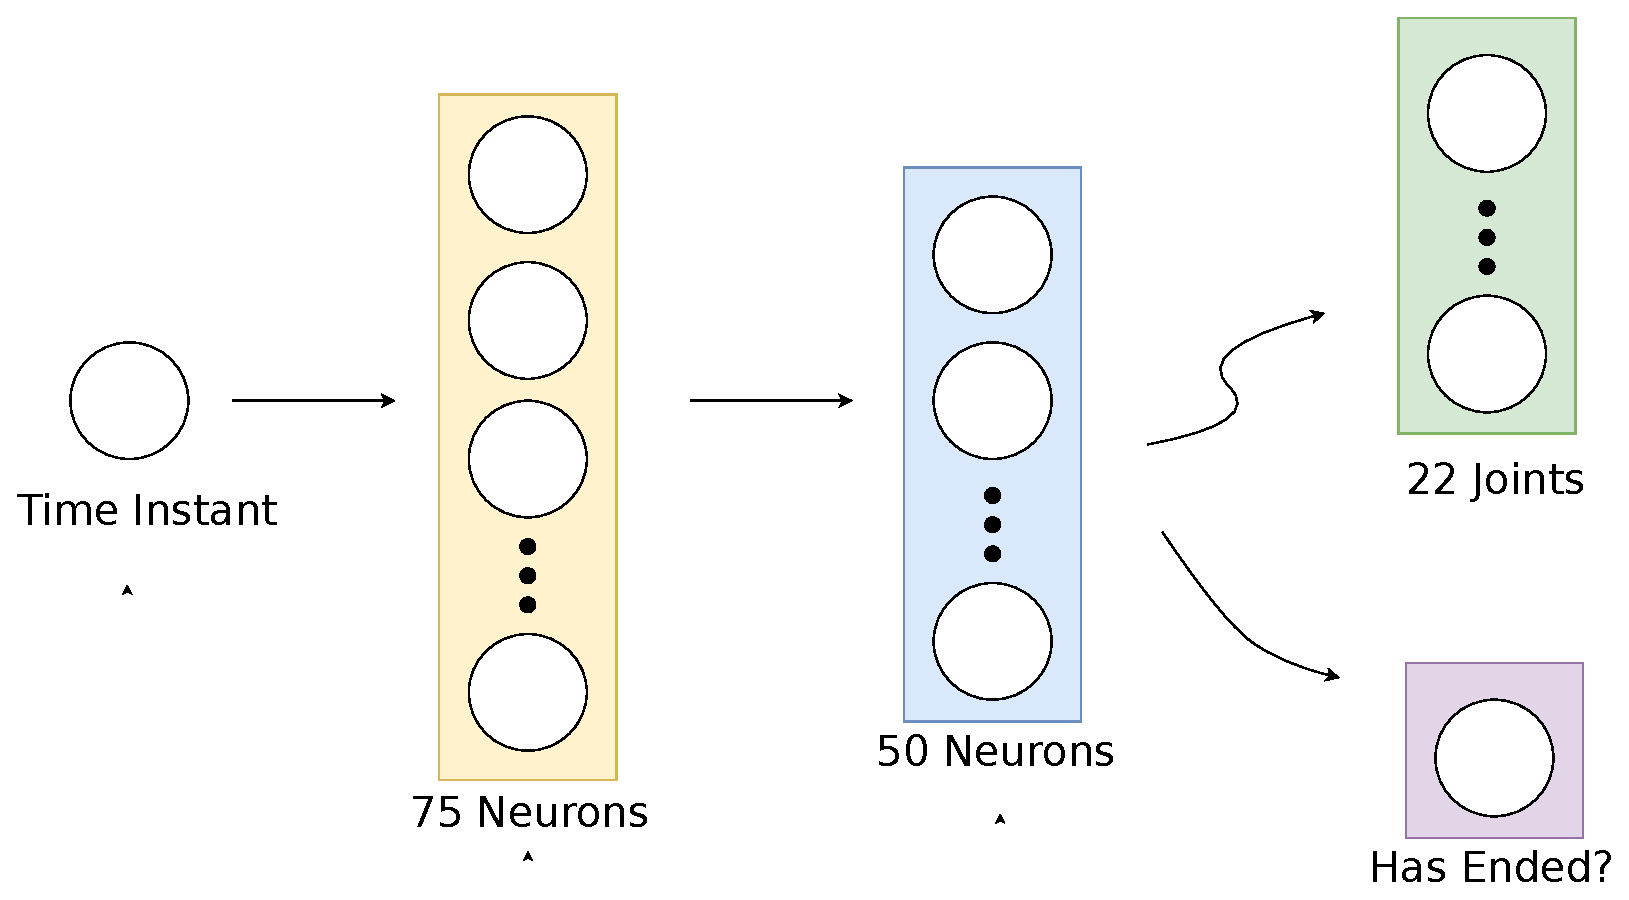
\includegraphics[width=0.5\textwidth]{Cap5/architecture}
\caption{The architecture of a neural network designed to learn motions.}
\label{fig:model_plot}
\end{figure}

This architecture resulted in thousand of parameters to optimize, as exposed in Table \ref{tab:network_summary}. A very high number, when compared to more traditional optimization approaches \cite{AAAI12-MacAlpine}. Notice that, by increasing the number of parameters usually allows representing better movements.

\begin{table}[htbp]
\caption{The Network Summary}
\begin{center}
\begin{tabular}{|c|c|c|c|}
\hline
\textbf{Layer}&{\textbf{Neurons}}& \textbf{Activation}& \textbf{Parameters} \\
\hline
Dense & 75 & LeakyReLU & 150  \\
\hline
Dense & 50 & LeakyReLU & 3800 \\
\hline
Dense & 23 & Linear & 1173 \\
\hline
\end{tabular}
\begin{tabular}{|c|c|}
\hline
\textbf{Total Parameters} & 5123 \\
\hline
\end{tabular}
\label{tab:network_summary}
\end{center}
\end{table}


\subsection{The Training Procedure}
Since keyframe motions are executed in an open-loop fashion, the sequence of joint positions are always the same for different repetitions, independently of robot's state. Therefore, by adding samples of multiple executions of the same motion would not make our dataset richer. So, we decided to use only one repetition for each movement for faster training. In the case of the walking motion, we collected samples within one walking period.

During the training, we used 50 thousands epochs divided into 5 training phases, where the learning rate was decreased between phases, in order to achieve better performance. First, we executed 30000 epochs, by using the learning rate of 0.001. The other phases had 5000 epochs each, and we decreased the learning rate by 0.0002 in each phase.

Furthermore, we used Adam optimization \cite{adam2014}, during the whole training. The loss function used was the mean squared error, as explained in Subsec. \ref{sec:neural_networks}. We decided this loss function is adequate for this problem, mainly because it strongly penalizes large errors, which can collapse the whole motion.

\subsection{The Deployment in the Soccer 3D Environment}
In order to perform the network design and the training procedure, we used the Keras \cite{chollet2015keras} framework coupled with Tensorflow \cite{tensorflow2015-whitepaper} as backend. After training, the weights were frozen and converted to a specific format, which was readable, by using the Tensorflow C++ API integrated within agent's code. Hence, the training was performed outside the environment, but the agent actually has computed network inferences, during the simulation execution.

\section{Reinforcement Learning Setup}

To use a Reinforcement Learning model, we need to define a policy representation and a task which the agent will follow during the process.

\subsection{Policy Representation}

The policy is represented by a neural network similar to the supervised learning model. A state is described as the stage of kick motion. An action is a set of joint values that has to be applied by the agent in that state.

In HLM, the architecture from both value function and policy networks is that described by section \ref{supervised_learning_setup}. On the other cases, the network is composed by three building blocks: an input normalization Filter, the neural networks themselves and a Gaussian action space noise.

\subsubsection{Input Normalization Filter}
The input normalization filter, also know as feature scaling, has the objective of normalize the input to avoid the problem of vanishing and exploding gradients by applying updates through all dimensions in equal proportions, as illustrated in Figure \ref{inputnormfig}. This normalization happens at each pass in the network, re-calculating mean and standard deviation using the new examples. Hence, this method helps during the convergence.

\begin{figure}[!htbp]
	\centering
	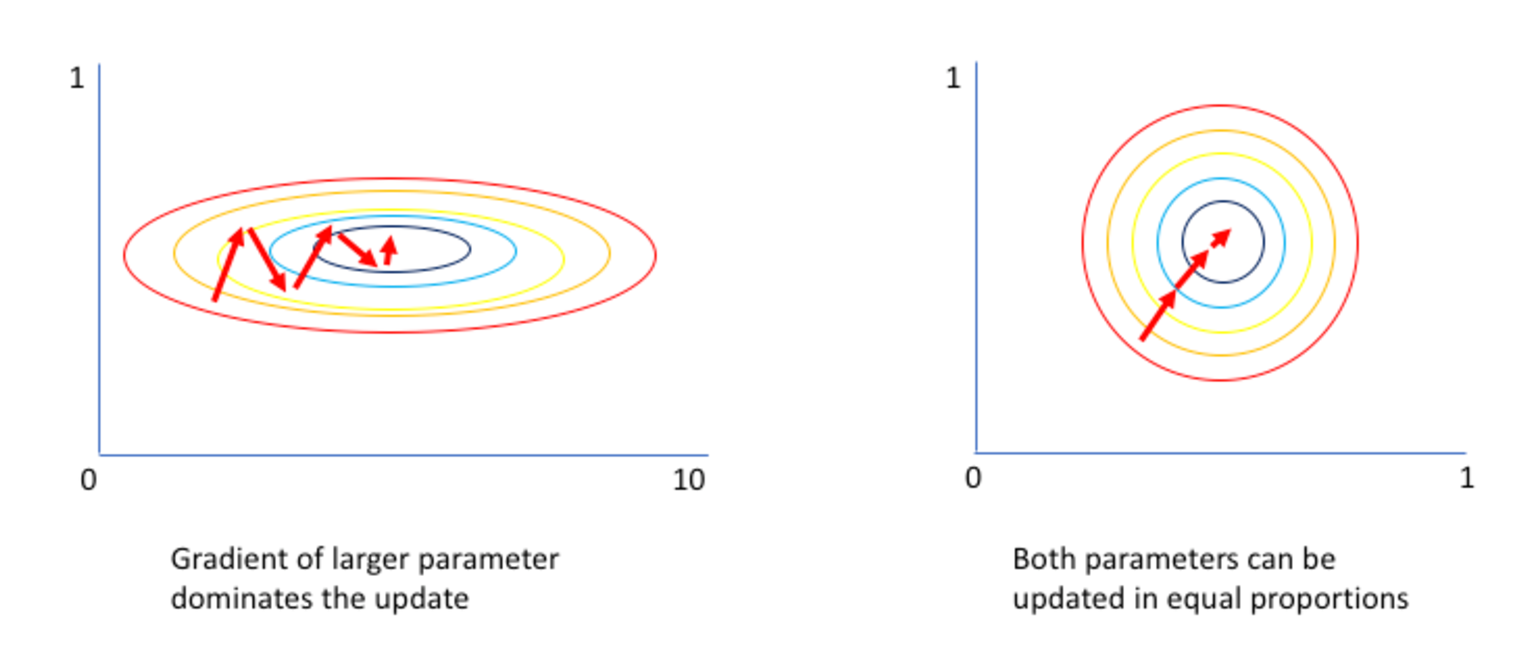
\includegraphics[width=0.5\textwidth]{Cap5/inputnorm.eps}
	\caption{Intuition behind input normalization}
	\label{inputnormfig}
\end{figure}

\subsubsection{Neural Network}
As an actor-critic model, we have two networks: one for the value function and other for the policy itself. They have the same architecture: two layer, fully connected, with 64 neurons in each hidden layer and hyperbolic tangent as activation function. The architecture is illustrated in Figure \ref{rlnetwork}. Table \ref{tab:rl_network_summary} summarizes the parameters in this new architecture, also considering the parameters from the Gaussian Action Space Noise, described in \ref{gasp}.

\begin{figure}[!htbp]
	\centering
	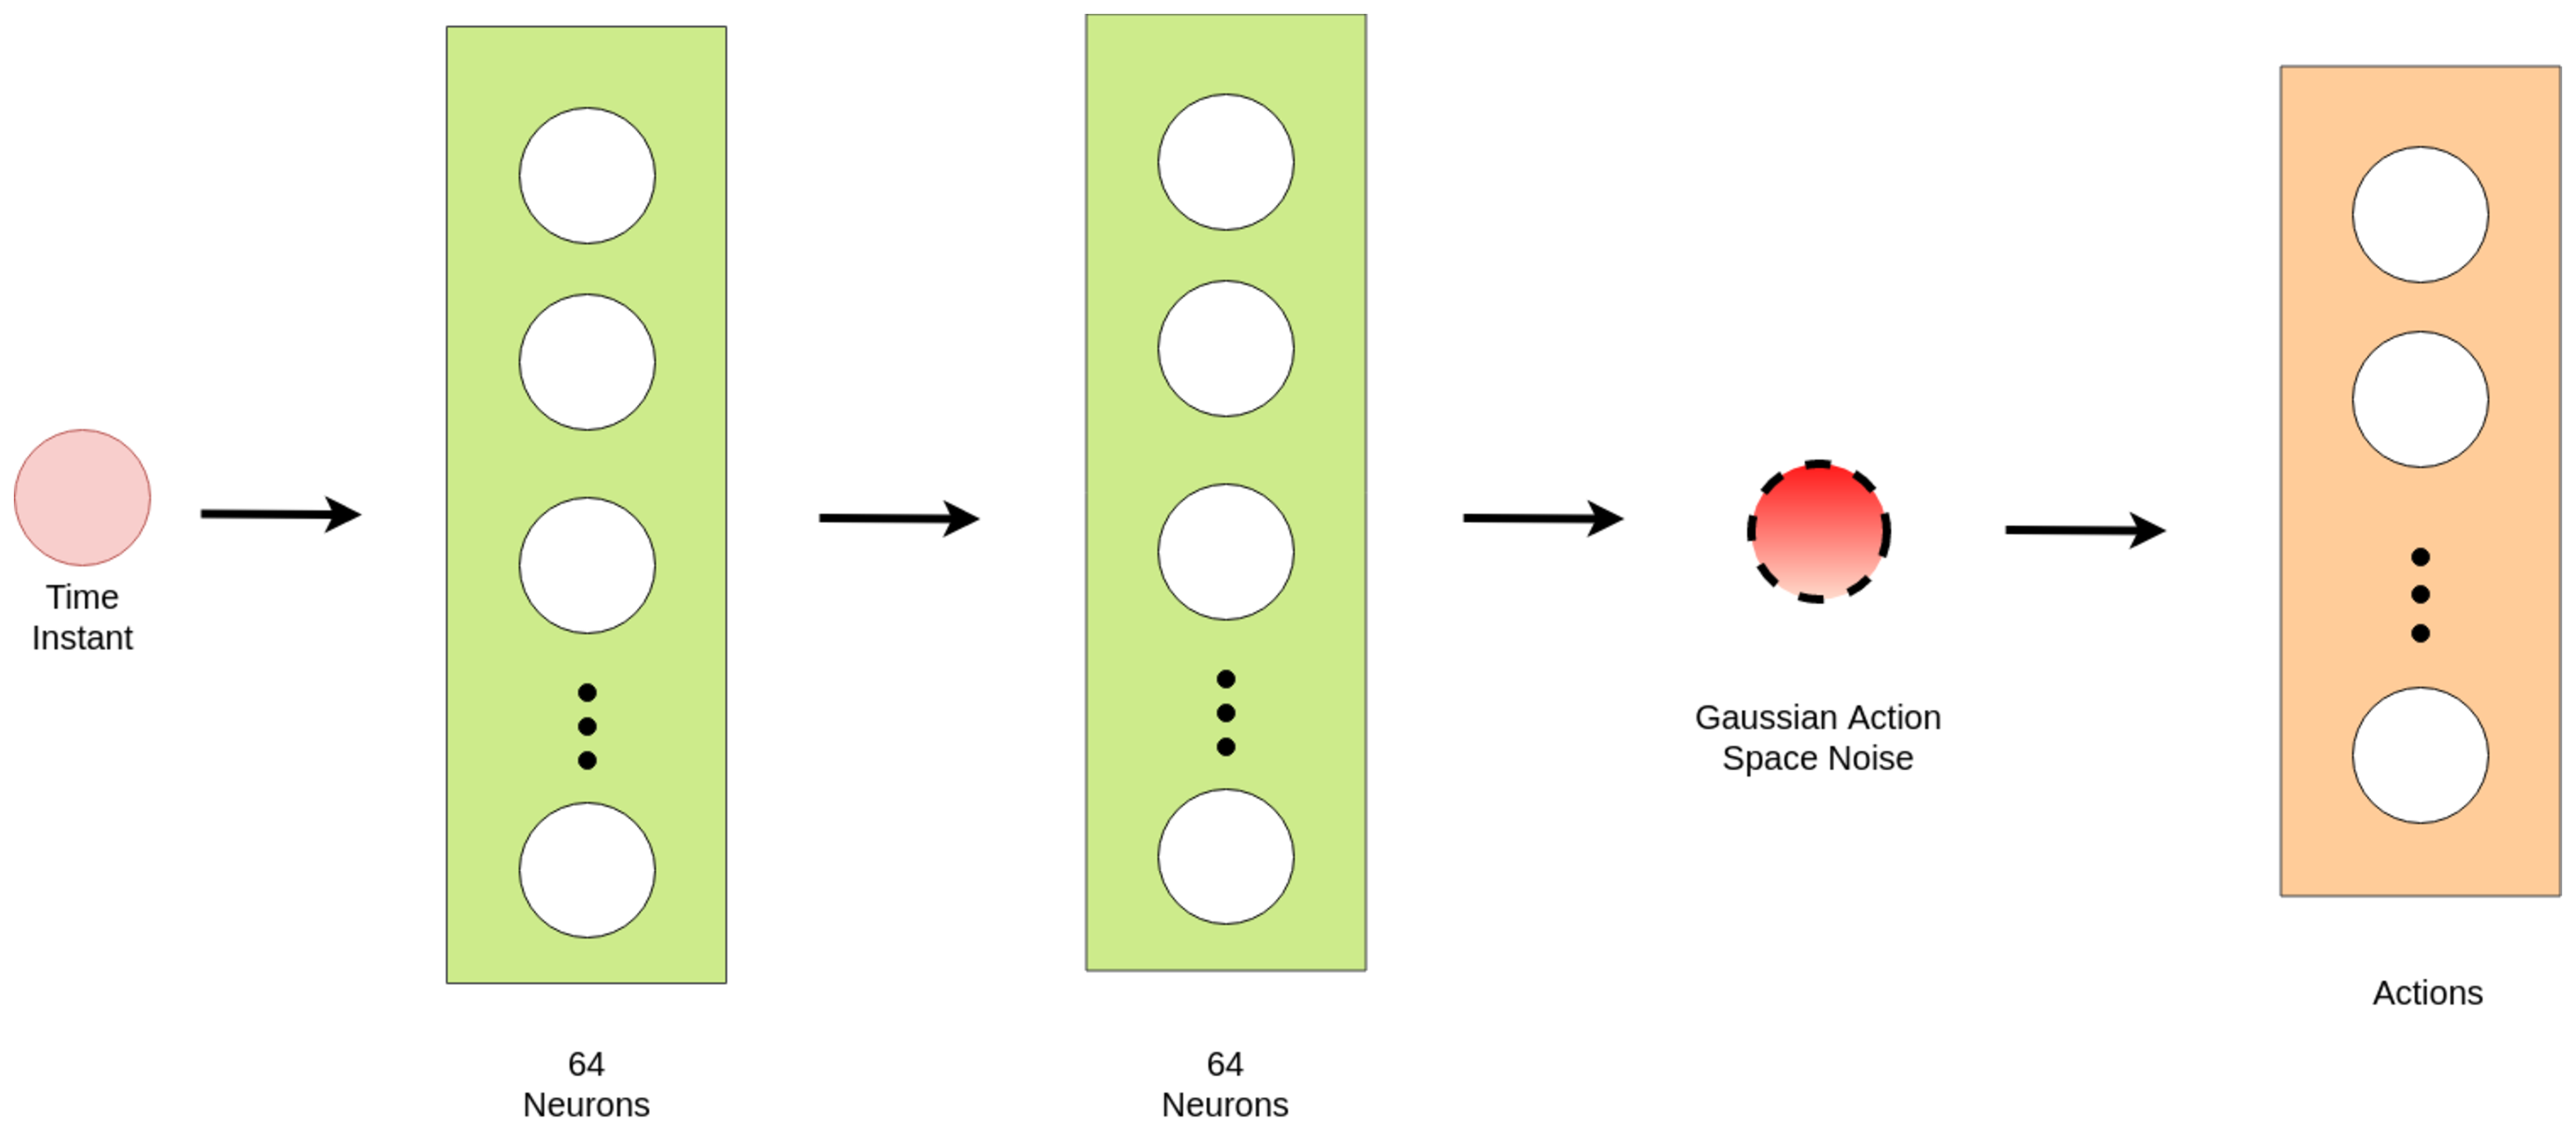
\includegraphics[width=0.5\textwidth]{Cap5/rlnetwork.eps}
	\caption{Architecture used by pure Reinforcement Learning models.}
	\label{rlnetwork}
\end{figure}

\begin{table}[htbp]
	\caption{The Reinforcement Learning Network Summary}
	\begin{center}
		\begin{tabular}{|c|c|c|c|}
			\hline
			\textbf{Layer}&{\textbf{Neurons}}& \textbf{Activation}& \textbf{Parameters} \\
			\hline
			Dense & 64 & $tanh$ & 128  \\
			\hline
			Dense & 64 & $tanh$ & 4160 \\
			\hline
			Output & 23 & Linear & 1495 \\
			\hline
			Noise & 23 & Linear & 23 \\
			\hline
		\end{tabular}
		\begin{tabular}{|c|c|}
			\hline
			\textbf{Total Parameters} & 5806 \\
			\hline
		\end{tabular}
		\label{tab:rl_network_summary}
	\end{center}
\end{table}


\subsubsection{Gaussian Action Space Noise}\label{gasp}

The last idea explored in this policy representation is the Gaussian action space noise for better exploration. It adds adaptive noise to the action space of the neural network. Discrete RL uses $\epsilon$-greedy \cite{Watkins:1989} to confer exploration. Gaussian action space noise injects normal randomness directly into the actions of the agent, altering the types of decisions it makes and helping algorithms explore continuous environments more effectively. The Figure \ref{gaussiannoise} illustrates this technique.


\begin{figure}[!htbp]
	\centering
	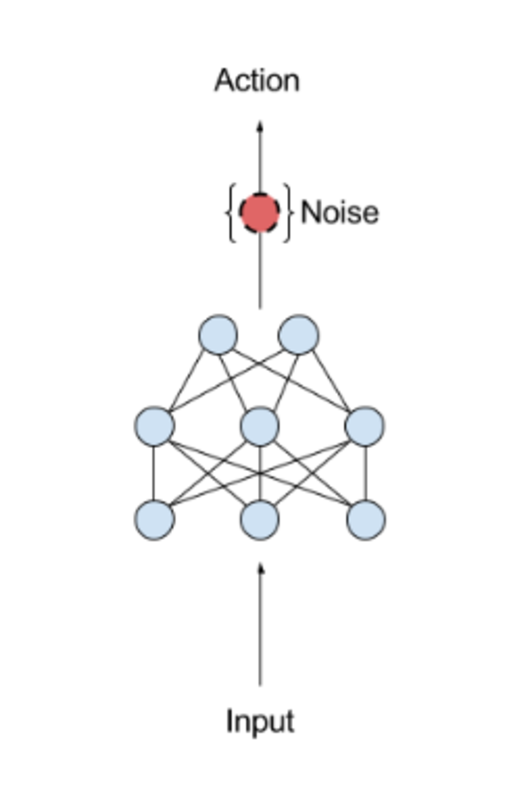
\includegraphics[width=0.3\textwidth]{Cap5/gaussiannoise.eps}
	\caption{Gaussian noise applied to action space to ensure better exploration in continuous environments.
	\cite{parameternoiseblog}
	}
	\label{gaussiannoise}
\end{figure}

\subsection{Task Description}
Image from roboviz executing the task.

\section{Infrastructure}